\section{Structure of the source code}

\subsection{Microservices}
Here the code regarding the microservices architecture is explained. \\
The source code that meets the requirements mentioned above has been organized in the following way: for each microservices a project
has been set up. 
Indeed, when dealing with this type of architecture, one should think of a microservice
as a project that should be as much independent as possible from the others: this is the reason that stands behind the choice that has been
made. 
Of course, in this way, it is possible to easily generate the single jars that will be deployed, when necessary, with, as mentioned
in the design document, dockers. Therefore, the following projects are present: API gateway, service registry, group individual request
service, individual request service and share data service. 
As one may notice, the one containing the set up of the API gateway also accesses all the information related with the accounts, and, therefore, authentication and authorization functions are coded here.
In the following sections the structure of the single projects are analyzed. 

\subsubsection{API Gateway}
In the figure ~\ref{fig:pkgapigateway}, it is shown the root of the project structure. An analysis 
of the various elements follows below the figure. 
\begin{figure}[H]
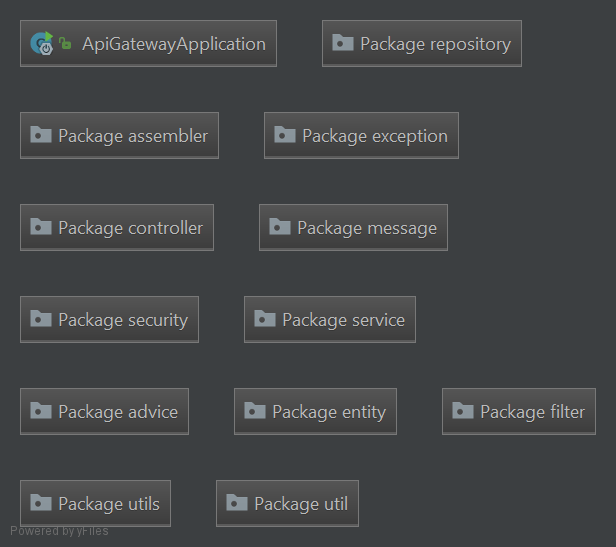
\includegraphics[width=\linewidth]{images/PackageApigateway.png}
\caption{ API gateway }
\label{fig:pkgapigateway}
\end{figure}

\begin{itemize}
\item Package repository: contains the JPA repository for accessing the persistent data necessary to this
service. 
In particular information regarding the accounts of users and third party customers are present. For what concerns the third party customers,
since they can register both as private and as related with a company the following repositories are present: company details, private
details, third party customers and users. An additional repository is present, and it accesses information regarding the API. Indeed, all
the accessible APIs that are available are stored in a database, in order to provide access control. For better specifying this choice, 
one may consider the fact that it is not necessary to search on the service registry non-existing API or to forward requests that can
be already classified as rejected (e.g. user A that is trying to access an API available only for third party customers)
\item Package assembler: this class contains components useful to build HATEOAS resources of entities that are returned to clients, adding
hypermedia contents
\item Package exception: this contains the custom exceptions defined during the development
\item Package controller: contains the controller that defines the APIs that regards the management of the users and third party customer
accounts. From here, it is possible to access the business functions that regards the account (e.g. login, logout, registration). Inside here,
controller are split into secure and public controllers: the public one are accessible to everyone, while for accessing the secured ones,
it is necessary to perform the log in
\item Package message: it provides the functions of communicating with other microservices, by means of RabbitMQ. In particular, three
subpackages are present here. The package publisher contains classes that helps in publishing the events of creation of new accounts to other 
services. The package protocol defines a way of communicating the interested pieces of information, and, finally the configuration
package specifies the configuration settings needed to convert object from JSON (and viceversa) during the propagation of data and also RabbitMQ exchanges and queues\cite{rabbit-concepts} .
\item Package security: contains the main features that have been introduced above regarding the security 
\item Package service: contains the services that implements the business functions of the account service, with all the APIs that it exposes.
The interfaces present here map the component interfaces of the account service
\item Package advice: this encompasses the handling of server side exceptions in order to show to clients useful messages without exposing
the structure of the project and low level errors
\item Package entity: here classes that are mapped to the databases are present   
\item Package filter: it includes filters that the API gateway applies during the management of "external" requests (i.e. requests that
need to be processed by other services). In particular, it is further subdivided into three packages: pre, route and post. In this case, the
pre filter that is present perform access control on the external API that is being requested, the route filter is a translation filter
that adds header in order to identify the clients in the other microservices, and the post filter fixes the hypermedia content that is sent
as a response to the original request
\item Package util: various utility needed in the development
\end{itemize}

The routes to the other microservices available are present in the application.properties file.
Here it follows a list of the API available:
\begin{itemize}

\item /public/users/authorize \\
This requires two request parameters, that are username and password. This API is necessary to login the users.
The method is POST.

\item /public/users/\{ssn\} \\
This is the entry point for registering a new user. Here, ssn is a path variable that specifies the social security number
of the user that will register. A request body that specifies the necessary fields of the JSON are specified in the user entity. \\
Here it is reminded that one should check the needed fields paying attention also to the defined JSON views defined. \\
This holds also for the other methods in which a request body is needed. \\
The method is POST.


\item /public/thirdparties/authorize \\
This requires two parameters, that are email and password. This API is necessary to login the third party customers. 
The method is POST.

\item /public/thirdparties/companies is necessary to register a third party customer that is related with a company. \\
A request body is needed to specify all the information related to that customer. The method is POST.

\item /public/thirdparties/privates is necessary to register a third party customer that is not related with a company.
A request body is needed to specify all the information related to that customer. The method is POST.

\item /users/info returns the information of the user that is accessing that API. The method is GET.

\item /users/logout performs the logout of the user from the system. The method is POST.

\item /thirdparties/info returns the information of the third party customer that is accessing the method. The method is GET.

\item /thirdparties/logout performs the logout of the third party customer from the system. The method is POST.

\end{itemize}


\subsubsection{Service registry}
The project of the service registry is almost empty, no package is present, but just an application class annotated with 
@EnableEurekaServer. The configuration of the service registry is set in the application.properties file.

\subsubsection{Group request service}
In the next figure, the package diagram of the group request project is shown ~\ref{fig:pkggrouprequest}. \\
The same comments hold here except for the fact that the business function mapped in the component interfaces are the one regarding
the group request service. 

\begin{figure}[H]
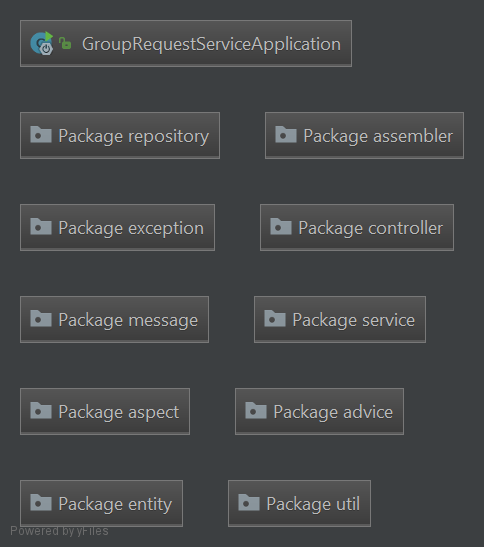
\includegraphics[width=\linewidth]{images/PackageGrouprequestservice.png}
\caption{ Group request service }
\label{fig:pkggrouprequest}
\end{figure}

Here it follows a list of the API available:
\begin{itemize}

\item /grouprequestservice/grouprequests/id/\{id\} \\
It retrieves the information related with the group request specified by the id in the
path variable. 
The method is GET.

\item /grouprequestservice/grouprequests/thirdparties \\
It collects all the group requests related with the third party that is accessing the method. 
The method is GET.

\item /grouprequestservice/grouprequests/thirdparties \\
This adds a new group requests. It requires a request body that contains all the details of the group
request that will be added.
The method is POST.

\end{itemize}

The prefix /grouprequestservice is necessary in order to access the APIs from the API gateway. 
Note, that by inspecting the controller, the prefix won't be shown at all: this is because the API gateway does this translation 
and mapping autonomously. Instead, one may notice some request headers: they are added at runtime by the gateway, and so the client
does not have to specify them, and, if it does, they will be overwritten. \\
This comment holds, as well, for all the other microservices.


\subsubsection{Individual request service}
Here it follows the package diagram of the individual request service project ~\ref{fig:pkgindividualrequest}. 
As one may notice, the structure is very similar to the one explained in the api gateway project. 
Of course, here, the controllers provide access to the APIs that regards the individual request service. 
The business functions of this project are present in the  service package, and the interfaces that are present, 
are mapped with the component interfaces of the Design document. \\
Another difference w.r.t. the API gateway that is worth to point out is that here the package message contains also a subpackages that
defines listeners: these are charged of listening to new events that are forwarded from RabbitMQ. 

\begin{figure}[H]
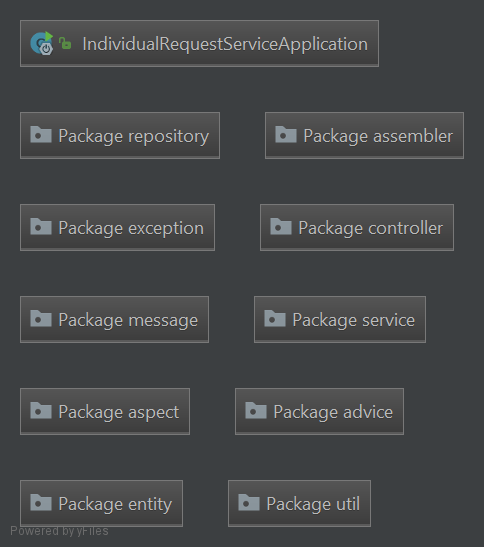
\includegraphics[width=\linewidth]{images/PackageIndividualrequestservice.png}
\caption{ Individual request service }
\label{fig:pkgindividualrequest}
\end{figure}

Here it follows a description of the available API:
\begin{itemize}
\item /individualrequestservice/requests/id/\{id\} \\
This retrieves an individual request identified by means of a certain id. 
The method is GET.

\item /individualrequestservice/requests/users \\ 
This retrieves the pending requests of the user that is accessing the method. 
The method is GET.

\item /individualrequestservice/requests/thirdparties \\ 
This retrieves the requests performed by the third party customer that is accessing the method.
The method is GET.

\item /individualrequestservice/requests/\{ssn\} \\
This adds a new individual request toward the user specified in the path variable.
A request body specifies the information requested to define the individual request.
The method is POST. 

\item /individualrequestservice/responses/requests/\{requestID\} \\
It is used in the case in which the user that is accessing the method
sends a response to the request identified by requestID in the path variable.

\item /individualrequestservice/responses/blockedThirdParty/thirdparties/\{thirdParty\} \\
It is used in the case in which the user that is accessing the method blocks the third party identified by the id specified in the path variable
\end{itemize}

\subsubsection{Share data service}
The structure of the share data service, as shown by the following picture, is also very similar to the previous ones 
~\ref{fig:pkgsharedata}.

\begin{figure}[H]
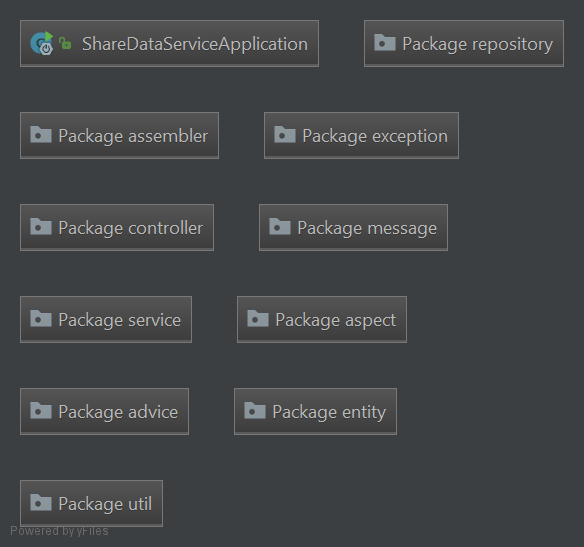
\includegraphics[width=\linewidth]{images/PackageSharedataservice.png}
\caption{ Share data service }
\label{fig:pkgsharedata}
\end{figure}

However, it is important to point out the structure of the code that manages the personalized query specified by the group requests on 
anonymized data. Basically, the custom query is realized with the help of QueryDSL, a sort of unified library to make queries; this choice comes from a limitation of Spring JPA: the impossibility to make union with dynamic queries. Therefore, after researches of other libraries supporting JPA, the best one and mostly supported by the community was QueryDSL which offers a method to makes JPA SQL queries. First of all it is necessary to say that JPA creates connection between objects of classes  and tuples of the DB; this has great advantages when it comes to use only JPA, but mixing it with other methods of retrieving data such as raw SQL queries could introduce some inconsistency. But thanks to JPA SQL queries it was possible to avoid this problem. In conclusion, the custom query is generally something with this simplified template:
\begin{itemize}
\item SELECT AGG\_OP(Column) FROM User JOIN ON Union(HealthData dynamic filtered, PositionData dynamic filtered) WHERE (sameSSN) AND "other filters of User table"
\end{itemize}
  
Here it follows a list of the main API that have been developed in the project, and that are located
within the various microservices.
It is possible to find these mapping in the controller packages. \\
The methods are expressed from a client point of view: for example, takes into consideration the methods that starts with s 

Here it follows a description of the available API

\begin{itemize}
\item /sharedataservice/dataretrieval/individualrequests/\{request\_id\} \\
This method retrieves the data related to the individual request identified by the path variable. The method is GET.

\item /sharedataservice/dataretrieval/grouprequests/\{request\_id\} \\
This method retrieves the data related to the group request identified by the path variable. The method is GET.

\item /sharedataservice/dataretrieval/users \\
This method retrieves the own data of the user. In this case, two request parameters
are necessary in order to specify an interval of time that involves the interested data.
The method is GET.

\item /sharedataservice/datacollection/healthdata \\
This allows the user to send data regarding the health status to the system. The method is POST.
A request body that specifies the data required.

\item /sharedataservice/datacollection/positiondata \\
This allows the user to send data regarding his position data to the system. The method is POST.
A request body that specifies the data required.

\item /sharedataservice/datacollection/clusterdata \\
This allows the user to send cluster of data (both health and position data). The method is POST.
A request body that specifies the data required.

\end{itemize}



\subsection{Mobile code}

\subsubsection{Data4Help}
The source code of the mobile application has been divided in different packages.
The main idea is to build an application where each component represents a microservice's view: 
they are loaded dynamically and they are assembled for drawing the complete user interface. 
This solution, even if it uses a monolithic approach, works well for relative simple mobile applications and it is more easy to implement. 
Of course, in this way, it is possible to easily generate the single APK that will be installed on the mobile device. \\
It follows an analysis that will focus on what is a service component and how it has been implemented in the code. 
In the project, a user interface component is a container, that is represented by an activity class. 
This classes follow the MVP pattern with delegation, thus allowing to have activities less complex and well structured, since the base
structure of an android application with the only uses of simple activities is a bad practice.
The MVP pattern is matched against the baseUtility package and his main components are: contract (basePresenterInterface and
baseViewInterface),
basePresenter, baseActivity and baseDelegate. \\
The fragment that truly represents the microservice's view are loaded into the activities. 

\begin{figure}[H]
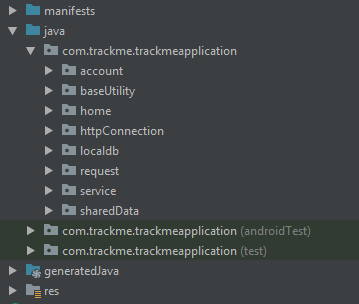
\includegraphics[width=\linewidth]{images/ProjectStructure.png}
\caption{ Code structure}
\label{fig:pkgsharedata}
\end{figure}

In the following paragraph the structure of each package is analyzed.

\paragraph{Account}
In the next figure, it is shown the account package structure and, after that, comes an explanation of the single parts.
  
\begin{figure}[H]
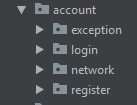
\includegraphics[width=0.6\linewidth ]{images/PackageAccount.png}
\caption{ Package account}
\label{fig:pkgsharedata}
\end{figure}

\begin{enumerate}
\item Package exception: this contains the custom exceptions defined during the development for the account service.
\item Package login: this contains the activity for the user login and the third party login. 
The user login is also the first activity when the application starts. 
It saves the user context in a persistent way by means of SharedPreferences class, and it requires the user all the permission that the
application needs to work properly, like: access to the location, internet, call phone, bluetooth and the possibility of writing on external
storage.
\item Package network: this package contains the account controller called accountNetworkInterface that exposes all the functions for the
communication with the account service on the server side.
\item Package register: here all the register forms are implemented to allow third parties (i.e. company and private third party) and
users to register into the application. 
\end{enumerate}

\paragraph{Base Utility}
The package base utility contains the implementation of the MVP pattern and the main utility used in the application. 
Furthermore, it contains the constant class with all the useful constants.

\paragraph{Home}
The home package contains the two main activities of the application. 
The UserHomeActivity shows the home view to the user, with the possibility of switching through three fragments: the home fragment that allows
the user to see his last health status, by pressing the check status button; the history fragment with all the health data registered in the 
last week; and, finally, the request fragment that allows the user to see the individual requests received and to accept or refuse some of
them. \\
The user home provides also a lateral menu, with the logout function and the possibility of activating two services: health and location
service. 
Note that the user settings and the user profile are only fake options, added for the completeness of the menu, but they are not so important,
and therefore they have not been implemented: more time has been devoted to other pieces of functionality. Also Term and Condition is a fake view. \\
The second activity that is present in this package is the business home: it is similar to the first, but it is composed of only two
fragments: one for showing to third parties the individual requests that they have sent and allow them create additional requests, and a
second one that does the same, but for the group requests.\\
In this package the synchronization between the slider that activates health and location service with the running of the service itself has
not been implemented since it is not so important to the prototype application.

\paragraph{HTTP Connection}
This package contains the main class for supporting a secure connection with the server. 
Connection thread is the only way to connect to the server and it loads, for all the connections, the SSL context with the certificate and the 
host verifier that checks if the server IP corresponds to an address known. 

\paragraph{Local db}
The structure of the local db realized with Room framework is now exposed.

\begin{figure}[H]
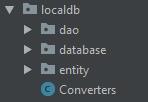
\includegraphics[width=0.6\linewidth]{images/LocalDB.png}
\caption{ Package local db}
\label{fig:pkgsharedata}
\end{figure}

\begin{enumerate}
\item Package dao: It contains interfaces that maps java function in SQL query.
\item Package database: this class contains the database abstract class.
\item Package entity: here classes that are mapped to the databases are present 
\end{enumerate}

\paragraph{Request}
In this paragraph the request package is presented. 
This package implements the client side of individual request service and group request service.

\begin{figure}[H]
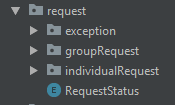
\includegraphics[width=0.6\linewidth]{images/Request.png}
\caption{ Package request }
\label{fig:pkgsharedata}
\end{figure}

\begin{enumerate}
\item Package exception: this contains the custom exceptions defined during the development.
\item Package individual request: here it is implemented the individual request user interface with fragments that can be loaded in the home
containers and the wrapper object that allows Object mapper to map immediately JSON strings to request objects. 
\item Package group request: same as above, but for group request. 
\end{enumerate}
	
\paragraph{Service}
In this package, the health service and the location service are implemented in order to receive data about health and position 
from, respectively, smartwatch or other similar devices and GPS. 
The application exploits the bluetooth functionality of the mobile device to receive the health data from the smartwatch, while for what 
concerns position data, it just receives it from the Location Manager of the device.\\

This package regards also AutomatedSOS and it is completely developed to work locally on the smartphone of the user. 

\begin{figure}[H]
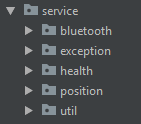
\includegraphics[width=0.6\linewidth]{images/Service.png}
\caption{ package service }
\label{fig:pkgsharedata}
\end{figure}

\begin{enumerate}
\item Package bluetooth: it contains a Bluetooth Server which is responsible of managing Bluetooth clients
\item Package exception: it contains all the custom exceptions used in the package
\item Package health: it contains the logic behind the health service which is based, basically, on the following: receiving the message;
saving the data if it is correct w.r.t. standard values; checking with simple threshold if the health is grave or not; if it is grave and
there are no recent emergency call, then it will get the user location and search for the emergency number within a JSON and call it
(afterwards, it saves the call on the local database to avoid flood calling)
\item Package util: it contains all the utilities class necessary for the health and position package. Here, it is important to  highlight the HealthDataInspectorImpl class in which it is defined the threshold of each field of health data:
\begin{itemize}
	\item heartbeat: the standard interval is $ [30, 220-age] $;
	\item minimum pressure: an interval of $ [40, 100]$;
	\item maximum pressure: an interval of $ [80, 200]$;
	\item blood oxygen level: it is a percentage of interval $ [80,100]$.
\end{itemize}
All these threshold are collected by an expert. If one of these thresholds are violated (excluded the case in which the health data is incorrect, i.e. bloody oxygen level not a percentage from 0 to 100), then the health data is considered to be grave and an emergency point should be called.
\item Package location: it contains the logic behind the location service, which just simply saves the position data on the local database
every time a new last location is present
\end{enumerate}

\paragraph{Share data}
Finally, the share data package is commented. 
The package structure is the same: it contains an exception package with the custom exceptions; it contains a network package with the
controller interface that exposes the function that allows the communication with share data service, and, finally, all the wrapper classes
for the mapping of the objects with JSON strings and vice versa.

\paragraph{Manifest folder}
This folder contains the application manifest that contains the properties of the application, like the definition of activities and user permission needed. 

\paragraph{Res folder}
Here are located all XML definitions files presented into the software. 
This files defines the aspect of the user interface and all the components styles.

\begin{figure}[H]
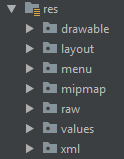
\includegraphics[width=0.6\linewidth]{images/Res.png}
\caption{ Res folder }
\label{fig:pkgsharedata}
\end{figure}

\begin{enumerate}
\item Package drawable: this package contains the XML definition of the drawable objects like images and icons.
\item Package layout: as the name says, it contains every activity layout. 
Note that the application is developed with automatically resizable layout and it supports portrait and landscape orientations.
\item Package menu: here there is the menu layout for the drawable menu on the left of the application.
\item Package mipmap: it contains the application icon.
\item Package raw: It contains two particular files. A JSON file with the last emergency call made by the user with Data4Help and keystore with the keys for secure communication.
\item Package value: here are stored string values, colors and component styles. 
\end{enumerate}

